\section{Conducting the Experiments}
\label{sec:Conducting_the_Experiments}
This section describes the experimental arrangement with the device list and all the measurement objects. Furthermore, it contains information about the measuring process. All measurements were conducted at 21 \textdegree C room temperature.

\subsection{Measurements}
\label{subsec:Measurements}
In this experiment, the following measurements were conducted:

\begin{enumerate}
	\item Wave length of sound waves in air, distilled water and aluminium for 1 kHz, 1 MHz and 5 MHz calculated from literature data
	\item Ultrasound velocity (longitudinal, reflection) for 1 MHz and 5 MHz in
	\begin{itemize}
		\item PMMA object
		\item Aluminium cylinder
		\item Copper cylinder
		\item Brass cylinder
	\end{itemize}
	\item Attenuation coefficient of PMMA for 1 MHz and 5 MHz
	\item Ultrasound velocity (longitudinal, reflection) for 5 MHz in
	\begin{itemize}
		\item Water at 20 \textdegree C
		\item Water at 50 \textdegree C
		\item Saltwater at 40 \textdegree C
	\end{itemize}
	\item Ultrasound velocity (transversal, reflection) for 1 MHz in PMMA
\end{enumerate}

\subsection{Experimental Arrangement}
\label{subsec:experimental_arrangement}
The experiment was arranged as shown below in figure \ref{fig:experimental_arrangement}:
\begin{figure}[H]
	\centering
	\includegraphics[scale=0.11]{experimental_arrangement}
	\caption{Annotated picture of the experimental arrangement for measurement no. 5: Ultrasound velocity (transverse, reflection) for 1 MHz in PMMA. For this measurement a special kind of ultrasound gel had to be used, as the transversal sound velocity was measured.}
	\label{fig:experimental_arrangement}
\end{figure}

\newpage
To measure the ultrasound velocity in water, a water bath and a reflector were used. This is shown in figure \ref{fig:experimental_arrangement_water_bath}:

\begin{figure}[H]
	\centering
	\includegraphics[scale=0.11]{experimental_arrangement_water_bath}
	\caption{Annotated picture of the experimental arrangement for measurement no. 4: Ultrasound velocity (longitudinal, reflection) for 5 MHz in saltwater at 40 \textdegree C. For this measurement the saltwater had to be heated up to the desired temperature with a heater and a magnetic stirrer.}
	\label{fig:experimental_arrangement_water_bath}
\end{figure}

The following equipment was used:

\begin{table}[H]
	\centering
	\renewcommand{\arraystretch}{1.2}
	\begin{tabular}{l l l}
		\hline
		\textbf{Device} & \textbf{Designation} & \textbf{Uncertainty} \\
		\hline
		Ultrasonic pulser / receiver unit & Olympus 5077PR (P-M5-025) & N/A \\
		Transducer 1 MHz (transverse) & Parametrics NDT V153 & N/A \\
		Transducer 1 MHz & Parametrics NDT V102 (892817) & N/A \\
		Transducer 5 MHz & Parametrics NDT V107 (900322) & N/A \\
		Oscilloscope & LeCroy WaveRunner 64MXi-A & $\pm0.05$ V / $\pm0.1\ \si{\mu s}$ \\
		Thermometer & Keithley 132C TRMS Multimeter & $\pm1$ \textdegree C \\
		Calliper & Mitutoyo CD-15PPX (13021983) & $\pm0.01$ mm \\
		Heater & IKA RCT basic (P-P8-052) & N/A \\
		Scale & OHAUS Scout Pro & N/A \\ \hline
	\end{tabular}
	\caption{List of the used equipment and measurement devices including test equipment number if available. Furthermore, the uncertainty is stated for all of the measurement devices (not for the regular equipment).}
	\label{tab:equipment}
\end{table}

\newpage
\subsection{Measurement Objects}
\label{subsec:measurement_objects}
The measuring objects are a range of different materials (PMMA, aluminium, copper, brass, water). The following figure \ref{fig:measurement_objects} shows the PMMA object, and the metal cylinders:

\begin{figure}[H]
	\centering
	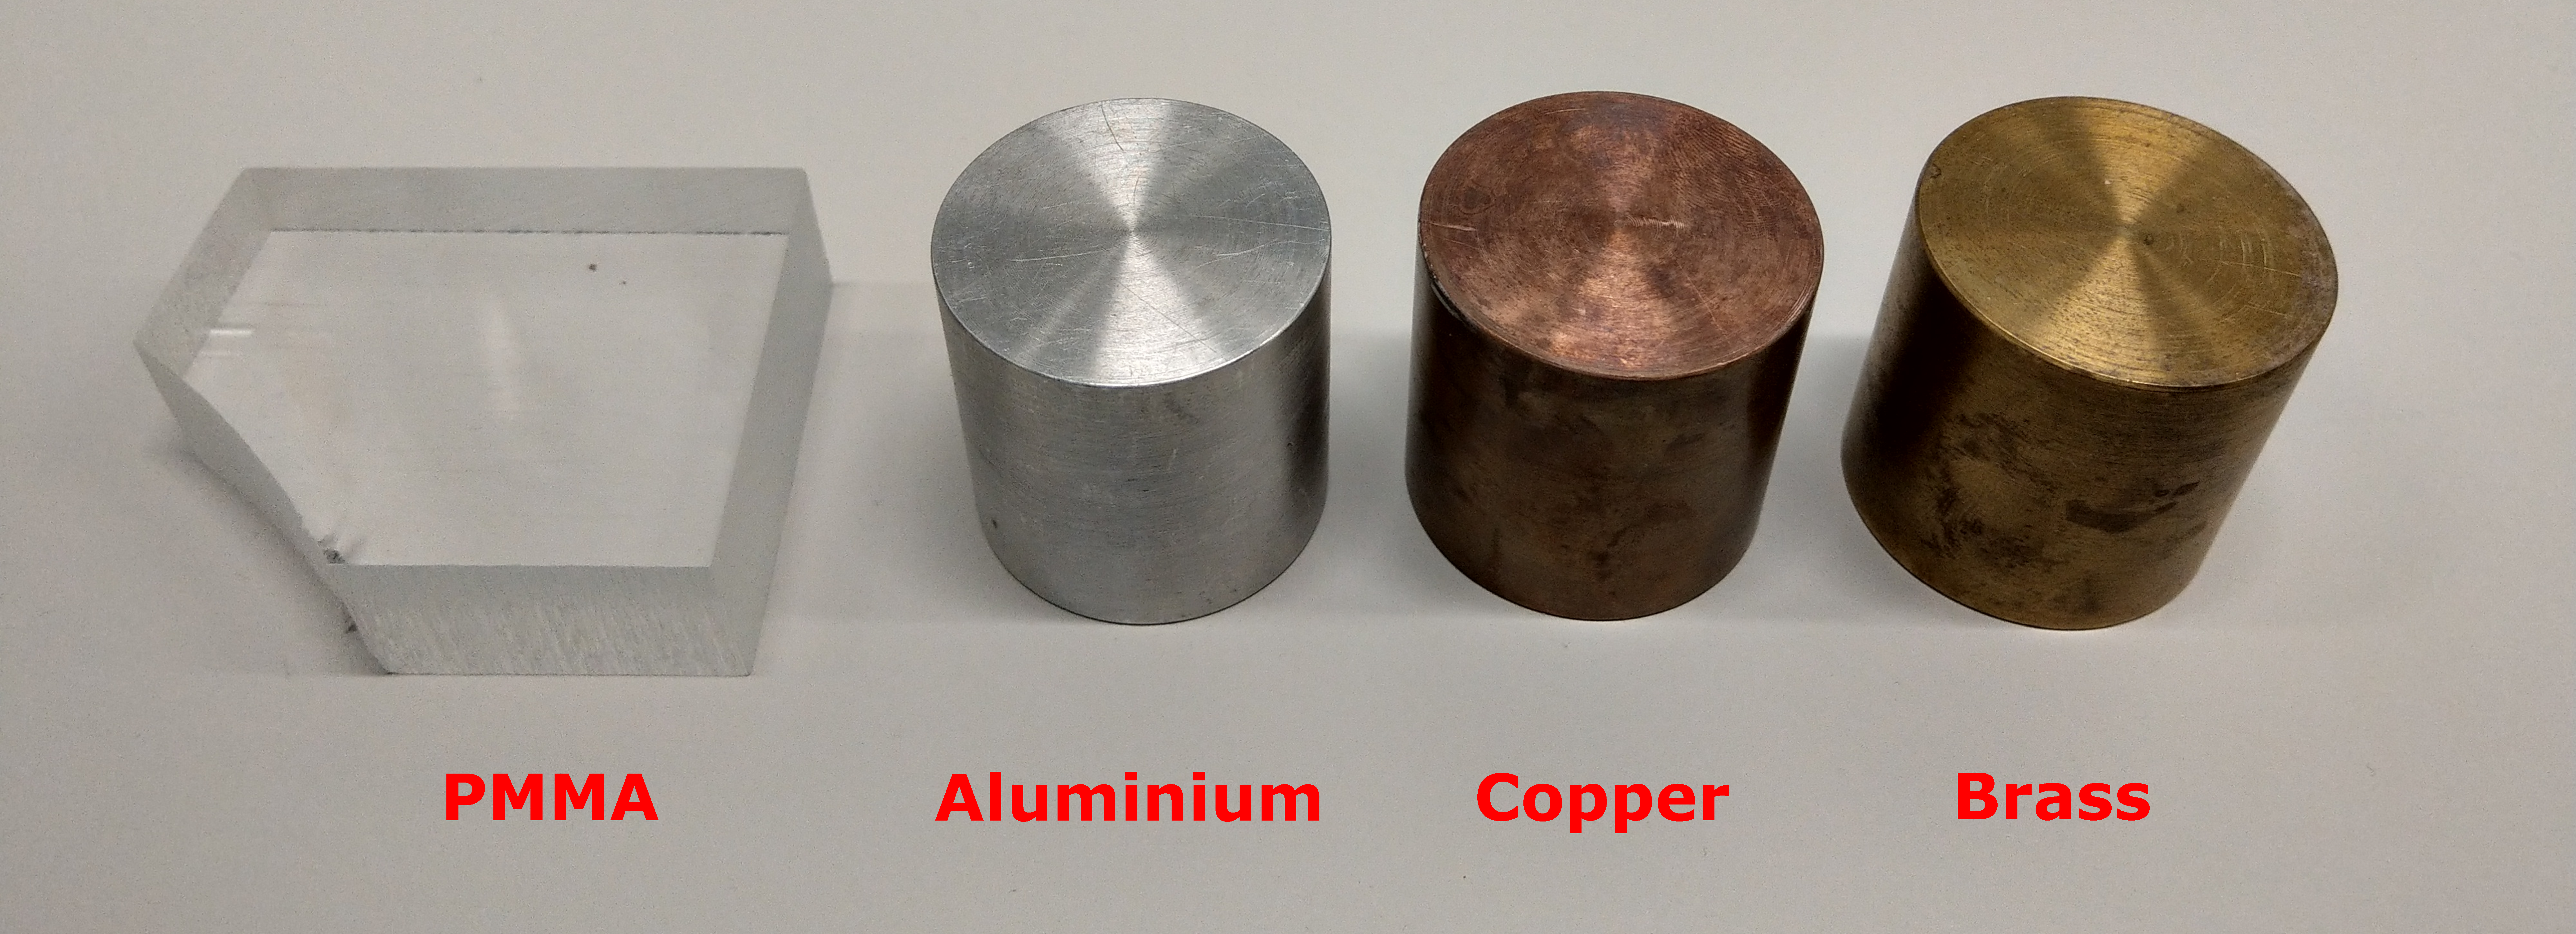
\includegraphics[scale=0.11]{measurement_objects}
	\caption{Annotated picture of the measurement objects used in measurements no. 2, 3 and 5. A PMMA object and three different metals (aluminium, copper and brass) were used.}
	\label{fig:measurement_objects}
\end{figure}

The different objects and their sound path distances are listed in the table \ref{tab:sound_path_distance} below.

\begin{table}[H]
	\centering
	\renewcommand{\arraystretch}{1.2}
	\begin{tabular}{r|l}
		 & \textbf{Sound Path Distance $x$} \\
		\hline
		\textbf{PMMA object} & $(20.40 \pm 0.01)\ \si{mm}$ \\
		\textbf{Aluminium cylinder} & $(40.03 \pm 0.01)\ \si{mm}$ \\
		\textbf{Copper cylinder} & $(40.05 \pm 0.01)\ \si{mm}$ \\
		\textbf{Brass cylinder} & $(40.06 \pm 0.01)\ \si{mm}$ \\
		\textbf{Water bath} & 0 mm up to $(180 \pm 0.1)\ \si{mm}$ \\ \hline
	\end{tabular}
	\caption{Specifications of the measured objects}
	\label{tab:sound_path_distance}
\end{table}

\subsection{Measuring Procedure}
\label{subsec:measuring_procedure}
The oscilloscope is connected to the ultrasonic pulser / receiver unit and shows the attenuated echoes received by the piezoelectric transducer. The time of flight (the duration it takes the sound wave to travel through the medium and return back to the transducer) is measured with the vertical cursors. Similarly, the amplitude is measured with the horizontal cursors. Figure \ref{fig:measuring_procedure} shows the waveform measured on the oscilloscope with a 5 MHz transducer in PMMA.

\begin{figure}[H]
	\centering
	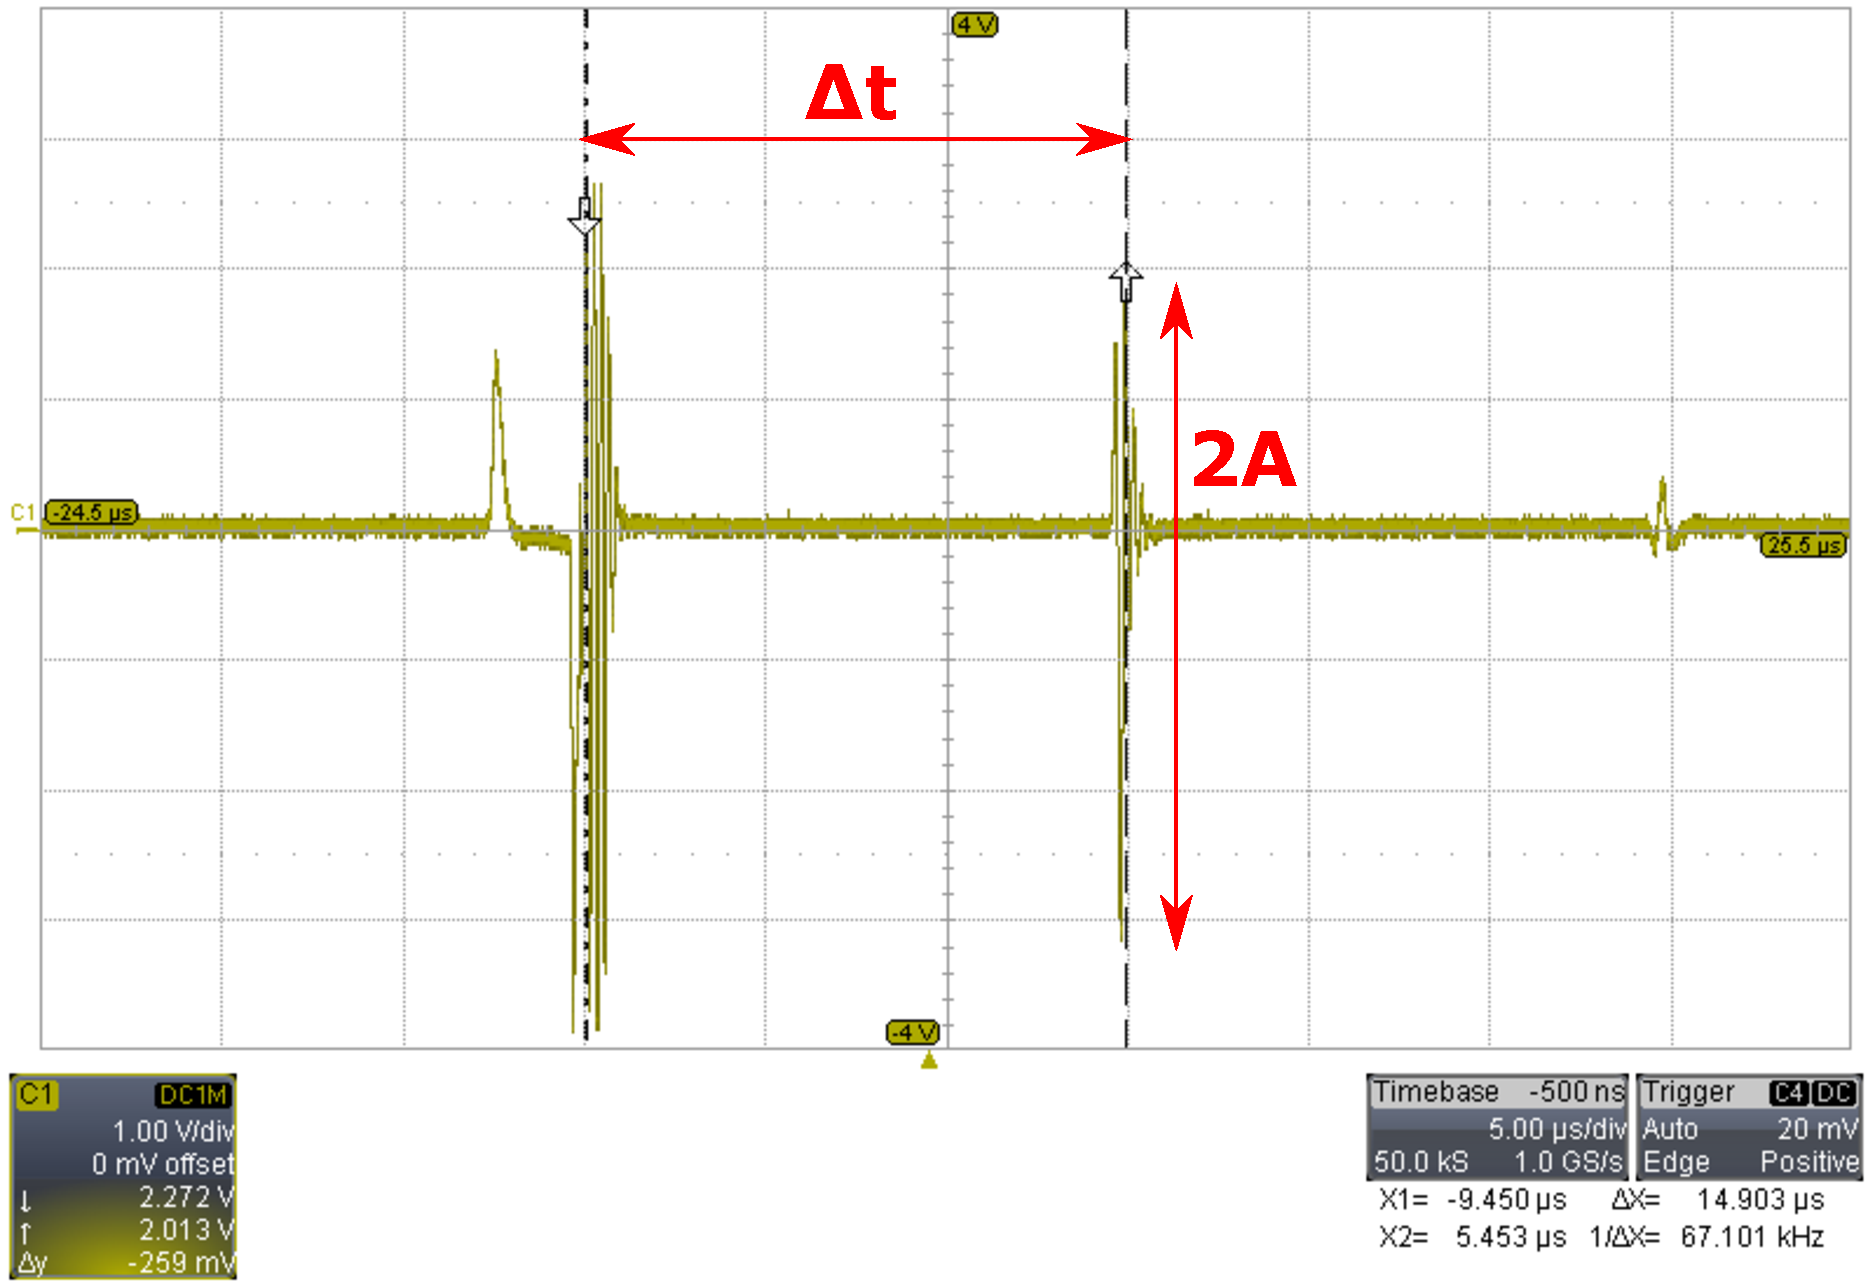
\includegraphics[scale=0.5]{measuring_procedure}
	\caption{Annotated picture of the waveform shown on the oscilloscope. The time of flight $\Delta t$ and the amplitude $A$ are marked in red. The peaks are the echoes that occur when the wave is totally reflected. The initial small peak is likely a reflection on the bottom plate of the piezoelectric transducer.}
	\label{fig:measuring_procedure}
\end{figure}
